\section{Proyectos}
\begin{itemize}
    \item Proyecto: Conjunto de actividades temporales para obtener un producto o un servicio. 
    \item PMBOK: Project Management Body of Knowledge (PMP)
    \item Hito: Resultado medible atemporal 
\end{itemize}

\begin{figure}[h!]
    \centering
        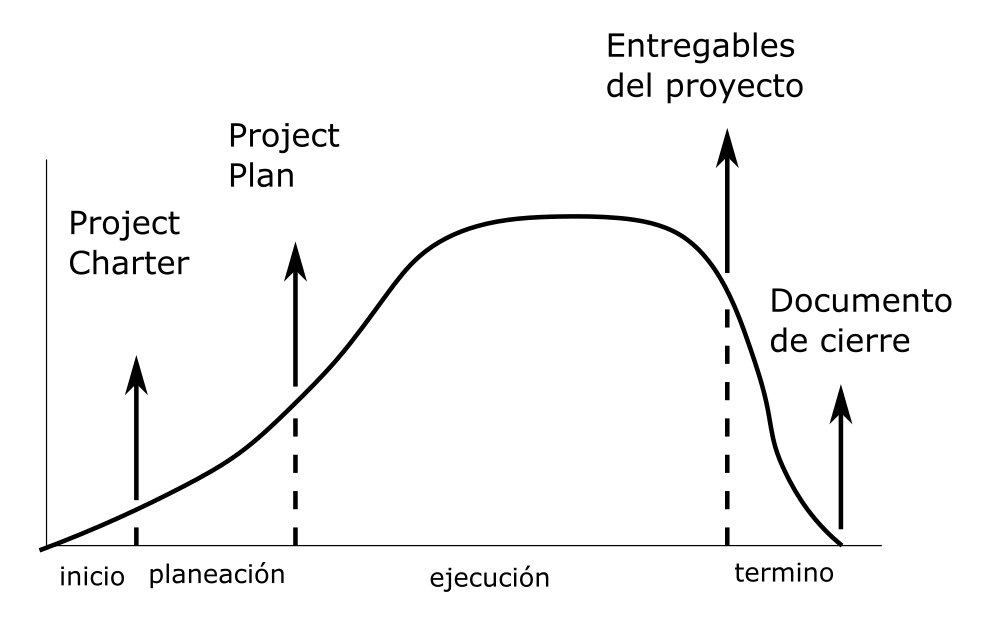
\includegraphics[scale=0.20]{Proyecto Integrador Figuras/04 Ciclo de Vida de Proyecto.png}
        \caption{Ciclo de vida de proyecto}
\end{figure}

\begin{figure}[h!]
    \centering
        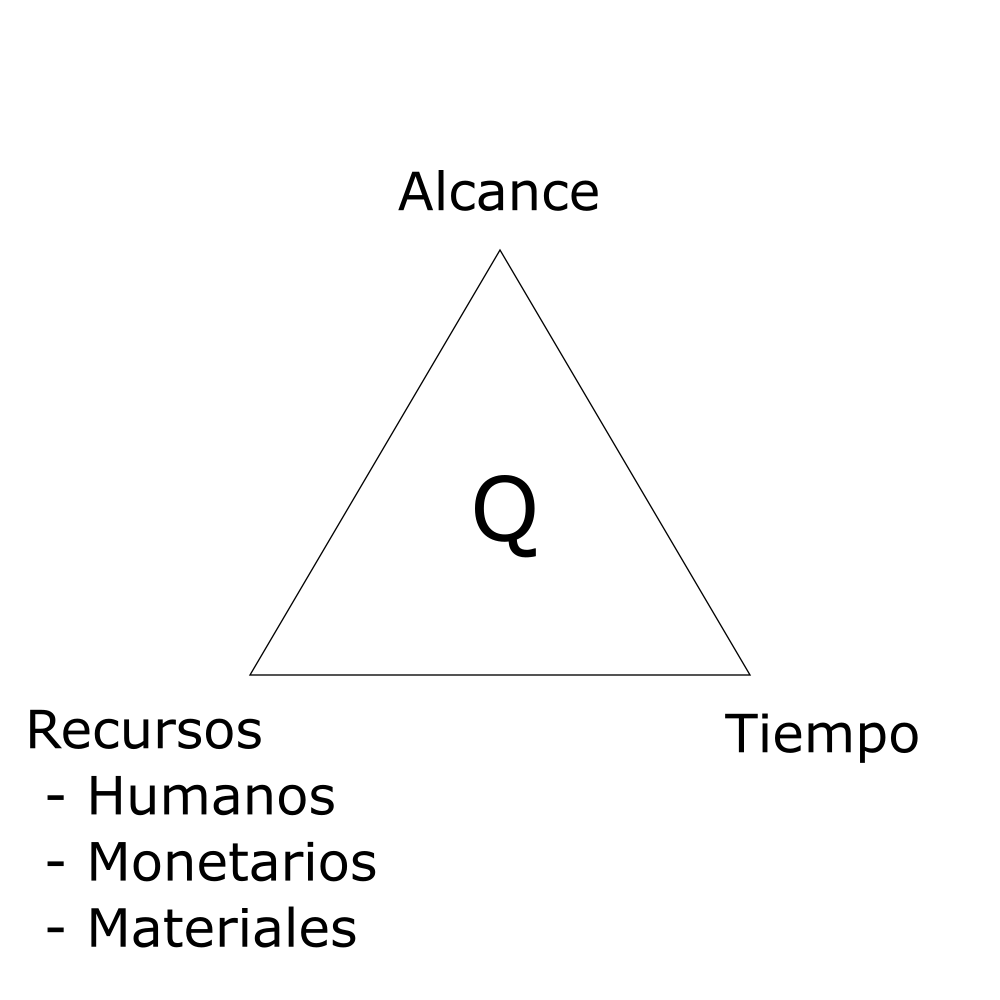
\includegraphics[scale=0.20]{Proyecto Integrador Figuras/05 Triangulo de Hierro.png}
        \caption{Triangulo de hierro}
\end{figure}